\documentclass[aspectratio=169]{beamer}

% Dependency setup
\usepackage{tikz}
%

% Beamer styling setup
\usetheme{AnnArbor}
\usecolortheme{beaver}
\setbeamercolor{titlelike}{parent=structure,bg=gray!15}
%

% Spacing setup
\setlength{\parindent}{0pt} % No paragraph indenting
\setlength{\parskip}{5pt} % Set spacing between paragraphs
\frenchspacing
\newcommand{\mkspace}{\vspace{19pt}}
\newcommand{\rmspace}{\vspace{-19pt}}
%
\usepackage{pgfpages}
\setbeameroption{show notes on second screen=right}

\begin{document}
\title{Paraméteres bonyolultság}
\author{Kovács Milán, Nemkin Viktória}
\date{2021. március 16.}

\frame{\titlepage}

\frame{\frametitle{Menetrend}\tableofcontents}

\section{Motiváció}

\begin{frame}
\frametitle{P nyelvosztály definíciója}

A P azoknak a nyelveknek az osztálya, amelyekhez van polinom időkorlátos
algoritmus (determinisztikus Turing-gép), azaz ha létezik olyan p(n) polinom, hogy
az algoritmus \textbf{az n méretű bemeneteken legfeljebb p(n)} lépést tesz.

Szeretnénk minden problémára polinom időkorlátos algoritmusokat adni...

Kérdés: Miért csak a bemenet hosszára figyelünk?

\end{frame}


\begin{frame}[t]
\frametitle{Példa: Prímtényezős felbontás}

Feladat: számok prímtényezős felbontását megadni.

\mkspace
\begin{columns}
\begin{column}{0.487\textwidth}
$4503599627370496 = 2^{52}$
\end{column}
\begin{column}{0.487\textwidth}
$1125897758834689 = 524287 \cdot 2147483647$
\end{column}
\end{columns}
\mkspace

\begin{itemize}
\item Input mérete: 16 számjegy.
\item Kézzel melyiket fogjuk tudni hamarabb megadni?
\item Számítógép: sokkal több számjegyre hasonlóan (pl. csak 10-nél kisebb prímek vannak benne $\leftrightarrow$ RSA kódolás).
\end{itemize}

\note{Ugyanolyan sok számjegyből állnak a számok, tehát ugyanolyan hosszú az input méretünk, mégis az elsőt
nagyon gyorsan meg lehet találni, a másodikat sokkal lassabban.}

\end{frame}


\begin{frame}
\begin{footnotesize}
\frametitle{Példa: Sűrű / ritka gráfok}
\note{Everything you want}

\begin{columns}
\begin{column}{0.5\textwidth}
Sűrű gráf:
\begin{center}
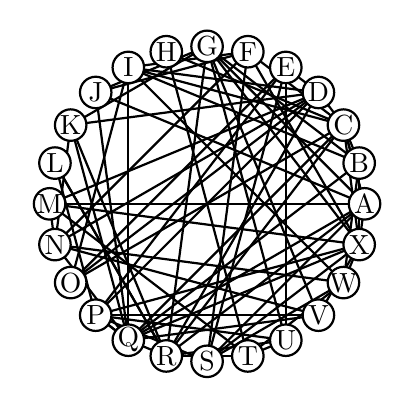
\begin{tikzpicture}[scale=2]
\coordinate (A) at (2.00000,1.00000);
\coordinate (B) at (1.96593,1.25882);
\coordinate (C) at (1.86603,1.50000);
\coordinate (D) at (1.70711,1.70711);
\coordinate (E) at (1.50000,1.86603);
\coordinate (F) at (1.25882,1.96593);
\coordinate (G) at (1.00000,2.00000);
\coordinate (H) at (0.74118,1.96593);
\coordinate (I) at (0.50000,1.86603);
\coordinate (J) at (0.29289,1.70711);
\coordinate (K) at (0.13397,1.50000);
\coordinate (L) at (0.03407,1.25882);
\coordinate (M) at (0.00000,1.00000);
\coordinate (N) at (0.03407,0.74118);
\coordinate (O) at (0.13397,0.50000);
\coordinate (P) at (0.29289,0.29289);
\coordinate (Q) at (0.50000,0.13397);
\coordinate (R) at (0.74118,0.03407);
\coordinate (S) at (1.00000,0.00000);
\coordinate (T) at (1.25882,0.03407);
\coordinate (U) at (1.50000,0.13397);
\coordinate (V) at (1.70711,0.29289);
\coordinate (W) at (1.86603,0.50000);
\coordinate (X) at (1.96593,0.74118);
\draw[thick] (B) -- (Q);
\draw[thick] (G) -- (V);
\draw[thick] (R) -- (U);
\draw[thick] (M) -- (X);
\draw[thick] (P) -- (P);
\draw[thick] (G) -- (U);
\draw[thick] (N) -- (M);
\draw[thick] (B) -- (I);
\draw[thick] (F) -- (N);
\draw[thick] (Q) -- (N);
\draw[thick] (A) -- (S);
\draw[thick] (N) -- (V);
\draw[thick] (X) -- (B);
\draw[thick] (B) -- (X);
\draw[thick] (J) -- (A);
\draw[thick] (T) -- (R);
\draw[thick] (F) -- (X);
\draw[thick] (N) -- (W);
\draw[thick] (V) -- (Q);
\draw[thick] (Q) -- (C);
\draw[thick] (R) -- (G);
\draw[thick] (Q) -- (R);
\draw[thick] (J) -- (F);
\draw[thick] (M) -- (D);
\draw[thick] (C) -- (H);
\draw[thick] (G) -- (A);
\draw[thick] (T) -- (U);
\draw[thick] (P) -- (Q);
\draw[thick] (H) -- (T);
\draw[thick] (P) -- (U);
\draw[thick] (C) -- (D);
\draw[thick] (S) -- (X);
\draw[thick] (S) -- (F);
\draw[thick] (X) -- (A);
\draw[thick] (I) -- (W);
\draw[thick] (I) -- (O);
\draw[thick] (I) -- (Q);
\draw[thick] (A) -- (C);
\draw[thick] (D) -- (O);
\draw[thick] (C) -- (A);
\draw[thick] (G) -- (J);
\draw[thick] (V) -- (X);
\draw[thick] (I) -- (D);
\draw[thick] (R) -- (D);
\draw[thick] (R) -- (C);
\draw[thick] (O) -- (E);
\draw[thick] (L) -- (P);
\draw[thick] (L) -- (R);
\draw[thick] (Q) -- (X);
\draw[thick] (W) -- (T);
\draw[thick] (E) -- (P);
\draw[thick] (K) -- (R);
\draw[thick] (S) -- (P);
\draw[thick] (U) -- (E);
\draw[thick] (V) -- (P);
\draw[thick] (R) -- (R);
\draw[thick] (E) -- (D);
\draw[thick] (B) -- (G);
\draw[thick] (M) -- (T);
\draw[thick] (N) -- (D);
\draw[thick] (D) -- (K);
\draw[thick] (X) -- (C);
\draw[thick] (C) -- (I);
\draw[thick] (N) -- (K);
\draw[thick] (A) -- (Q);
\draw[thick] (G) -- (X);
\draw[thick] (E) -- (S);
\draw[thick] (M) -- (A);
\draw[thick] (P) -- (X);
\draw[thick] (W) -- (S);
\draw[thick] (F) -- (I);
\draw[thick] (M) -- (M);
\draw[thick] (R) -- (A);
\draw[thick] (Q) -- (K);
\draw[thick] (R) -- (L);
\draw[thick] (Q) -- (P);
\draw[thick] (J) -- (Q);
\draw[thick] (P) -- (D);
\draw[thick] (G) -- (K);
\draw[thick] (W) -- (X);
\draw[thick] (C) -- (B);
\draw[thick] (W) -- (W);
\draw[thick] (F) -- (C);
\draw[thick] (O) -- (C);
\draw[thick] (H) -- (H);
\draw[thick] (W) -- (B);
\draw[thick, fill=white] (A) circle (0.1) node {A};
\draw[thick, fill=white] (B) circle (0.1) node {B};
\draw[thick, fill=white] (C) circle (0.1) node {C};
\draw[thick, fill=white] (D) circle (0.1) node {D};
\draw[thick, fill=white] (E) circle (0.1) node {E};
\draw[thick, fill=white] (F) circle (0.1) node {F};
\draw[thick, fill=white] (G) circle (0.1) node {G};
\draw[thick, fill=white] (H) circle (0.1) node {H};
\draw[thick, fill=white] (I) circle (0.1) node {I};
\draw[thick, fill=white] (J) circle (0.1) node {J};
\draw[thick, fill=white] (K) circle (0.1) node {K};
\draw[thick, fill=white] (L) circle (0.1) node {L};
\draw[thick, fill=white] (M) circle (0.1) node {M};
\draw[thick, fill=white] (N) circle (0.1) node {N};
\draw[thick, fill=white] (O) circle (0.1) node {O};
\draw[thick, fill=white] (P) circle (0.1) node {P};
\draw[thick, fill=white] (Q) circle (0.1) node {Q};
\draw[thick, fill=white] (R) circle (0.1) node {R};
\draw[thick, fill=white] (S) circle (0.1) node {S};
\draw[thick, fill=white] (T) circle (0.1) node {T};
\draw[thick, fill=white] (U) circle (0.1) node {U};
\draw[thick, fill=white] (V) circle (0.1) node {V};
\draw[thick, fill=white] (W) circle (0.1) node {W};
\draw[thick, fill=white] (X) circle (0.1) node {X};
\end{tikzpicture}
\end{center}

\end{column}

\begin{column}{0.5\textwidth}
Ritka gráf:
\begin{center}
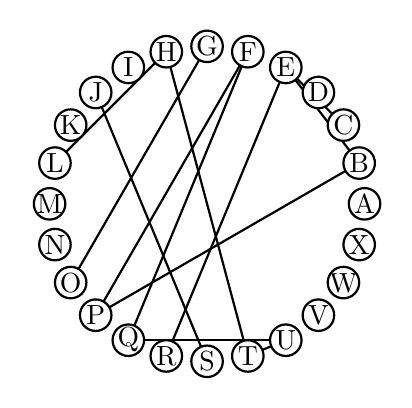
\begin{tikzpicture}[scale=2]
\coordinate (A) at (2.00000,1.00000);
\coordinate (B) at (1.96593,1.25882);
\coordinate (C) at (1.86603,1.50000);
\coordinate (D) at (1.70711,1.70711);
\coordinate (E) at (1.50000,1.86603);
\coordinate (F) at (1.25882,1.96593);
\coordinate (G) at (1.00000,2.00000);
\coordinate (H) at (0.74118,1.96593);
\coordinate (I) at (0.50000,1.86603);
\coordinate (J) at (0.29289,1.70711);
\coordinate (K) at (0.13397,1.50000);
\coordinate (L) at (0.03407,1.25882);
\coordinate (M) at (0.00000,1.00000);
\coordinate (N) at (0.03407,0.74118);
\coordinate (O) at (0.13397,0.50000);
\coordinate (P) at (0.29289,0.29289);
\coordinate (Q) at (0.50000,0.13397);
\coordinate (R) at (0.74118,0.03407);
\coordinate (S) at (1.00000,0.00000);
\coordinate (T) at (1.25882,0.03407);
\coordinate (U) at (1.50000,0.13397);
\coordinate (V) at (1.70711,0.29289);
\coordinate (W) at (1.86603,0.50000);
\coordinate (X) at (1.96593,0.74118);
\draw[thick] (T) -- (H);
\draw[thick] (Q) -- (U);
\draw[thick] (P) -- (F);
\draw[thick] (S) -- (J);
\draw[thick] (C) -- (E);
\draw[thick] (B) -- (P);
\draw[thick] (G) -- (O);
\draw[thick] (Q) -- (F);
\draw[thick] (E) -- (B);
\draw[thick] (H) -- (L);
\draw[thick] (E) -- (R);
\draw[thick] (T) -- (U);
\draw[thick, fill=white] (A) circle (0.1) node {A};
\draw[thick, fill=white] (B) circle (0.1) node {B};
\draw[thick, fill=white] (C) circle (0.1) node {C};
\draw[thick, fill=white] (D) circle (0.1) node {D};
\draw[thick, fill=white] (E) circle (0.1) node {E};
\draw[thick, fill=white] (F) circle (0.1) node {F};
\draw[thick, fill=white] (G) circle (0.1) node {G};
\draw[thick, fill=white] (H) circle (0.1) node {H};
\draw[thick, fill=white] (I) circle (0.1) node {I};
\draw[thick, fill=white] (J) circle (0.1) node {J};
\draw[thick, fill=white] (K) circle (0.1) node {K};
\draw[thick, fill=white] (L) circle (0.1) node {L};
\draw[thick, fill=white] (M) circle (0.1) node {M};
\draw[thick, fill=white] (N) circle (0.1) node {N};
\draw[thick, fill=white] (O) circle (0.1) node {O};
\draw[thick, fill=white] (P) circle (0.1) node {P};
\draw[thick, fill=white] (Q) circle (0.1) node {Q};
\draw[thick, fill=white] (R) circle (0.1) node {R};
\draw[thick, fill=white] (S) circle (0.1) node {S};
\draw[thick, fill=white] (T) circle (0.1) node {T};
\draw[thick, fill=white] (U) circle (0.1) node {U};
\draw[thick, fill=white] (V) circle (0.1) node {V};
\draw[thick, fill=white] (W) circle (0.1) node {W};
\draw[thick, fill=white] (X) circle (0.1) node {X};
\end{tikzpicture}
\end{center}

\end{column}
\end{columns}

Erre a két gráfra nézzünk gráfalgoritmusokat:
\begin{itemize}
\item Legnagyobb független csúcshalmaz.
\item Csúcsszínezés.
\item Stb...
\end{itemize}

Mindkét gráfban ugyanannyi csúcs van, ezért ha szomszédossági mátrixukkal adjuk meg őket, akkor
ugyanakkora lesz az input mérete, azonban a 2. gráfban a fenti kérdésekre elég hamar választ
tudunk adni.
\end{footnotesize}
\end{frame}


\begin{frame}
\frametitle{Valós életbeli problémák}

Üzleti korlátok:

\begin{itemize}
\item Facebook:
\begin{itemize}
\item ismerősök száma $\leq{}$ 500 (fokszám)
\item aktív felhasználók száma $\leq{}$ 3 milliárd (csúcsszám)
\end{itemize}
\item Google:
\begin{itemize}
\item keresett kifejezés hossza $\leq{}$ 100 karakter (illesztett minta hossza)
\item egy oldalon a linkek száma $\leq{}$ 1000 (fokszám)
\end{itemize}
\item Orvosi alkalmazások:
\begin{itemize}
\item DNS hosszúsága
\item protein max mérete
\end{itemize}
\end{itemize}
...stb
\end{frame}




\section{Bar Fight Prevention problem}
\begin{frame}
\frametitle{Feladat}

Sztori
\begin{itemize}
\item Biztonsági őr egy vidéki bárban
\item Péntek esti bulik: verekedés
\item Falu lakóit ismerjük, tudjuk ki kit nem szeret $\rightarrow$ ők verekedni fognak
\item Megelőzés: nem engedünk be olyanokat akik nem szeretik egymást
\item Menedzsment: profitmaximalizálás $\rightarrow$ legfeljebb k vendég elutasítása
\end{itemize}

Input
\begin{itemize}
\item Vendégek listája (n darab vendég)
\item Minden vendégpárra: szeretik-e egymást
\item Legfeljebb hány vendéget utasíthatunk el: k (kevesebbet lehet).
\end{itemize}

Output
\begin{itemize}
\item Megoldható-e úgy a feladat, hogy a beengedettek között ne legyen verekedés?
\item Kiket kell kitiltani?
\end{itemize}

\end{frame}


\begin{frame}
\frametitle{Példa: a szürkéket kell kidobni}
\begin{center}
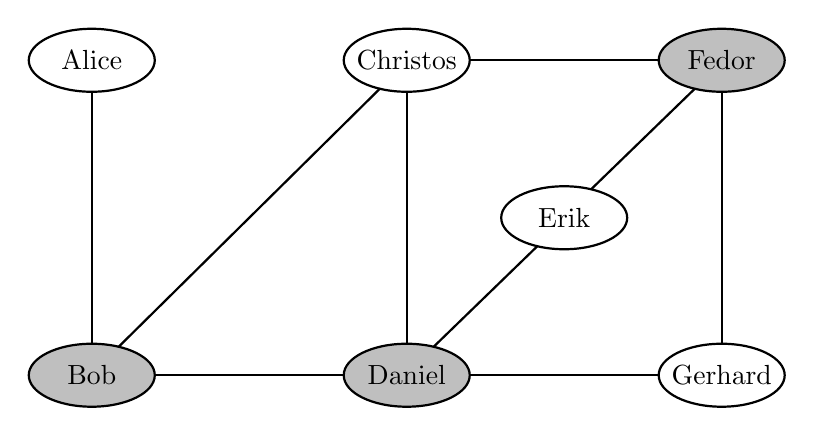
\begin{tikzpicture}[scale=2]
\draw[thick, fill=lightgray] (1,1) ellipse (0.4 and 0.2) node {Bob};
\draw[thick, fill=lightgray] (3,1) ellipse (0.4 and 0.2) node {Daniel};
\draw[thick] (5,1) ellipse (0.4 and 0.2) node {Gerhard};
\draw[thick] (4,2) ellipse (0.4 and 0.2) node {Erik};
\draw[thick] (1,3) ellipse (0.4 and 0.2) node {Alice};
\draw[thick] (3,3) ellipse (0.4 and 0.2) node {Christos};
\draw[thick, fill=lightgray] (5,3) ellipse (0.4 and 0.2) node {Fedor};

\draw[thick] (1.4,1) -- (2.6,1);
\draw[thick] (3.4,1) -- (4.6,1);
\draw[thick] (3.4,3) -- (4.6,3);

\draw[thick] (1,1.2) -- (1,2.8);
\draw[thick] (3,1.2) -- (3,2.8);
\draw[thick] (5,1.2) -- (5,2.8);

\draw[thick] (1.17,1.18) -- (2.83,2.82);
\draw[thick] (3.17,1.18) -- (3.83,1.82);
\draw[thick] (4.17,2.18) -- (4.83,2.82);

\end{tikzpicture}
\end{center}

\end{frame}


\begin{frame}
\frametitle{Megoldás}

\begin{center}
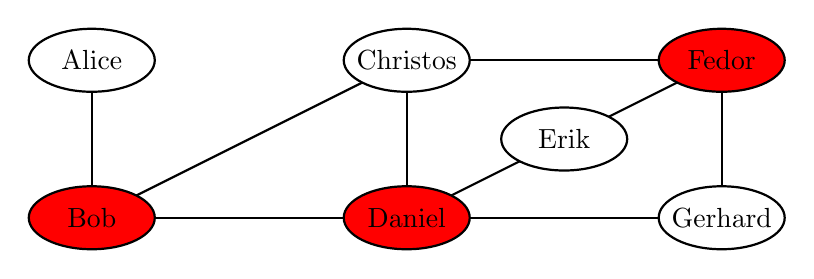
\begin{tikzpicture}[scale=2]
\coordinate (A) at (1,2);
\coordinate (B) at (1,1);
\coordinate (C) at (3,2);
\coordinate (D) at (3,1);
\coordinate (E) at (4,1.5);
\coordinate (F) at (5,2);
\coordinate (G) at (5,1);

\draw[thick] (B) -- (D);
\draw[thick] (D) -- (G);
\draw[thick] (C) -- (F);

\draw[thick] (B) -- (A);
\draw[thick] (D) -- (C);
\draw[thick] (G) -- (F);

\draw[thick] (B) -- (C);
\draw[thick] (D) -- (E);
\draw[thick] (E) -- (F);

\draw[thick, fill=white] (A) ellipse (0.4 and 0.2) node {Alice};
\draw[thick, fill=red  ] (B) ellipse (0.4 and 0.2) node {Bob};
\draw[thick, fill=white] (C) ellipse (0.4 and 0.2) node {Christos};
\draw[thick, fill=red  ] (D) ellipse (0.4 and 0.2) node {Daniel};
\draw[thick, fill=white] (E) ellipse (0.4 and 0.2) node {Erik};
\draw[thick, fill=red  ] (F) ellipse (0.4 and 0.2) node {Fedor};
\draw[thick, fill=white] (G) ellipse (0.4 and 0.2) node {Gerhard};
\end{tikzpicture}
\end{center}

\begin{footnotesize}
\begin{itemize}
\item Csúcsok = vendégek, élek = verekedni fognak.
\item Kitilható vendégek száma: k=3.
\end{itemize}
Kérdések:
\begin{itemize}
\item Kit tiltsunk ki, hogy ne legyen verekedés? \\
\textcolor{red}{Bob-ot, Daniel-t és Fedor-t.}
\item Melyik Algoritmuselméletből tanult feladat ez? \\
\textcolor{red}{k elemű lefogó csúcshalmaz: $\forall$ él legalább egyik végpontja benne van.}
\end{itemize}
\end{footnotesize}
\end{frame}


\begin{frame}
\frametitle{Brute force megoldás}
\begin{itemize}
\item Brute force algoritmus.
\item Minden lehetséges részhalmazt megnézzük: ha őket dobnánk ki a többiek verekednének-e?
\item $2^n$, pl n=1000-re már túl nagy.
\end{itemize}
\end{frame}


\begin{frame}
\frametitle{Ha tudjuk, hogy a k kicsi, pl. $k\leq{}10$}
\begin{itemize}
\item A menedzsment úgysem fog nagy k-t engedni.
\item Aki 0 fokszámú azt beengedhetem, mert senkivel nem fog összeveszni.
\end{itemize}
\end{frame}


\begin{frame}
\frametitle{Maradék gráf}

\begin{footnotesize}
\begin{itemize}
\item Csúcsok száma: $n$ (pl. $1000$)
\item Élek száma: $e$
\item Még kizárható vendégek száma: $k'\leq{}k$ (pl. $10$)
\item Csúcsok fokszáma: $1\leq{}d(v)\leq{}k'$
\end{itemize}
\end{footnotesize}

\begin{itemize}
\item Minden kitiltás $\leq{}k'$ konfliktust fog megoldani.\pause
\item Még $k'$ kitiltásunk maradt.\pause
\item Összesen $\leq{}k'^2$ konfliktust tudunk megoldani.\pause
\item $k'^2<e$ élre: nem megoldható, kész.\pause
\item $e\leq{}k'^2$ élre: csúcsok száma$\leq{}2k'^2$.\pause
\item ${2k^2 \choose k}$ mostmár $k\leq{}10$-re már jobb mint az előbbi $2^n$.
\end{itemize}
\end{frame}

\input{02_bar_fight_prevention_problem/07_1_k_foku_graf}
\begin{frame}
\frametitle{1 fokú csúcsok}
\begin{itemize}
\item Az 1 fokú csúcs és szomszédja esetében: ha beengedem a csúcsot akkor az 1 darab szomszédját nem engedhetem be.
\item Ezzel biztos nem lett rosszabb a helyzet, mert ha a csúcsot nem engedem be akkor a szomszédját beengedhetem, de annak még lehetnek egyéb szomszédjai is.
\item Ezért engedjük be az 1 fokú csúcsokat és tiltsuk ki a szomszédokat (ezzel k-t is csökkentsük 1-el).
\item Így mostmár 2..k konfliktus lehet.
\item Erre megint kiszámolom a max csúcsszámot, ez mostmár csak $k^2$, erre még jobb szám jön ki.
\end{itemize}
\end{frame}

\input{02_bar_fight_prevention_problem/09_1_fokszamu_valasz}
\input{02_bar_fight_prevention_problem/10_2_k_foku_graf}
\input{02_bar_fight_prevention_problem/11_bounded_search_tree}

\begin{frame}
\frametitle{?}
Itt van még a példának folytatása bounded search tree-kkel, de azt inkább Milánnak kellene elmondania.
\end{frame}

\begin{frame}
\frametitle{Kernelizációs technika általánosan}
\end{frame}


\begin{frame}
\frametitle{Vertex cover feladat megoldása egyben}
\end{frame}

\begin{frame}
\frametitle{Paraméteres komplexitás definíciója általánosan}
\end{frame}

\begin{frame}
\frametitle{Szemezgetés}
\end{frame}
\end{document}
